\begin{center}
\footnotesize\noindent\fbox{
	\parbox{\textwidth}{
	Relativamente al precedente esercizio, stimare numericamente la crescita della costante di Lebesgue.
	}
}\end{center}

\noindent Essendo le ascisse di interpolazione i nodi di Chebyshev, la costante di Lebesgue in fuzione di \(n\) si comporta come segue:
\[
\Lambda_n \approx \frac{2}{\pi}\log n
\]

\noindent Ci si aspetta quindi che abbia una crescita logaritmica al crescere di \(n\). Questo fatto \'e stato verificato calcolando le seguenti stime numeriche:

\begin{center}
	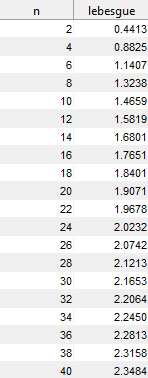
\includegraphics[scale=0.7]{cap4/4_8.png}
\end{center}

\noindent Il codice Matlab usato per realizzare la precedente tabella \'e il seguente:

\lstinputlisting[language=Matlab]{cap4/4_8.m}
